\section{x-project toolkit}
\brand{x-project} is a set of libraries and API-centric HTML5 Web Components based Web Application and CMS framework.



% \subsection{Philosophy}
``Everything is an element'', even an AJAX request. Every part of the website is encapsulated inside an element. Even functional components such as HTTP services (AJAX calls), pages and routing logic are encapsulated inside elements. We push Web Components' philosophy beyond all limits so that users can reach a very high level of customization and ease of use.

Component-based Software Engineering denotes the process of building software by (re)using pre-built software components. The main benefit of component-based software is the ``time-to-market'' \cite{4773208}, thus reducing the cost of developing the software. A software component is a unit of composition with contractually specified interfaces and explicit context dependencies. 
Additionally, a component is a software element that conforms to a component model and can be independently deployed and composed \cite{Heineman:2001:CSE:379381}. 
Component based software is developed interconnecting building blocks, therefore, a high degree of reusability and modularity is achieved by this type of applications \cite{914739}. 






\subsection{Client-side}

Client-side can be divided in two parts: \texttt{admin part} and \texttt{user part}.
\texttt{admin part} is automatically generated from the models schemas. It let the admin to manage (via CRUD operations) the models.
\texttt{user part} depends on the type of the Web Application that has been implemented.
It is the part the final user interact with.

% \begin{figure}[!htbp]
% \centering
% 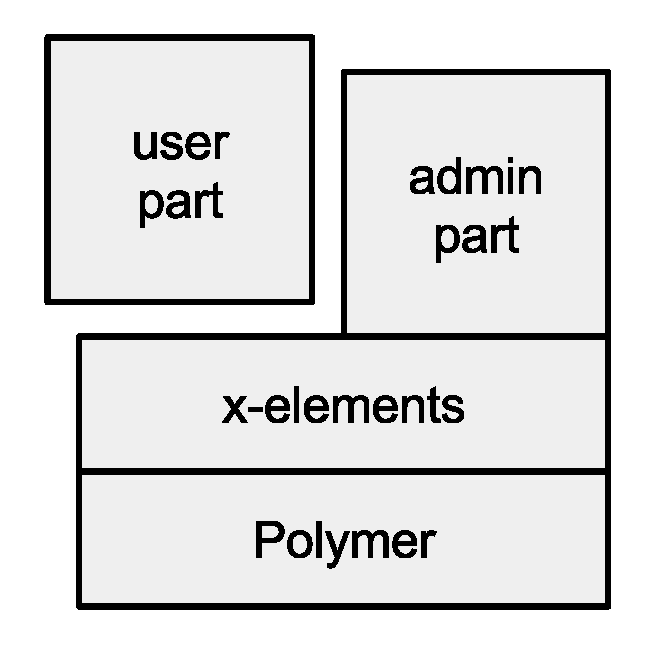
\epsfig{file=images/client-arch.eps, height=0.2\textwidth}
% \caption{Client-side architecture}
% \label{fig:client-arch}
% \end{figure}

\brand{x-project} provide a set of Polymer element for local routing, API requests, User management, forms composition, layout and style. 

\subsubsection{Elements for local routing}
\brand{x-project} provide elements to perform local routing to implement Single Page Application pattern.

\begin{description}
\itemsep1pt\parskip0pt\parsep0pt
        \item[\texttt{<x-router>}] implements local routing based on \emph{HTML5 Push State API}. 
        \item[\texttt{<x-route>}] represents a route-to-page mapping. It has two input attributes: \texttt{route} and \texttt{page}. A route can be parametrized: parameters are sent as attributes to the corresponding page.
        \item[\texttt{<x-link>}] is the extension of the native anchor element (\texttt{<a>}). It prevents the default behavior, blocking page request to the server and letting to manage the routing locally. 
\end{description}

\subsubsection{Elements for API requests}
\texttt{x-projects} provide a set of elements to handle collections and models API.

\begin{description}
\itemsep1pt\parskip0pt\parsep0pt
       \item[\texttt{<api-collection-get>}] retrieve a collection of models. It has input attributes to handle filters and pagination and an output attributes that stores the collection.
       \item[\texttt{<api-collection-post>}] add a new model to the collection. It has an input attribute that refers to the model to save.
       \item[\texttt{<api-collection-schema>}] retrieve a model schema.
       \item[\texttt{<api-model-(get|put|delete)>}] retrieve, update or delete a model. These have an input attribute that refers to the model.
\end{description}

For example, the following element perform an \texttt{HTTP GET} request to \texttt{/api/Posts} using filter and returning the first 10 items of the second page and the total number of items (helpful for pagination element).

\begin{lstlisting}[language=HTML5]
<api-collection-get name="Posts" 
  perpage="10" page="2" filter="{{filter}}"
  collection="{{posts}}" count="{{count}}">
</api-collection-get>
\end{lstlisting}


\subsubsection{Elements for User management}
\brand{x-project} provides a set of elements to manage User.
\texttt{<x-login>} is a form (with \texttt{email} and \texttt{password} input elements) that let the user login in the application. Once logged in, every API request is signed with a token that refers to the current user, for ACL reasons.


\subsubsection{Elements for forms composition}
\brand{x-project} provides a set of input elements to create forms. 

\texttt{<x-input>}, \texttt{<x-textarea>}, \texttt{<x-number>}, \texttt{<x-date>}, are respectively associated to short text, long text, number, and date; \texttt{<x-location>}, based on Google Place APIs, allows to choose locations using autocomplete add-on; \texttt{<x-file>}, based on the \brand{x-project} direct upload module, allows to upload files.
\texttt{<x-form>}, given a model schema, generates a form to edit models that match that schema; it is a composition of the input elements.

\subsubsection{Elements for layout and style}
\brand{x-project} provides a set of elements for layout, such as: \texttt{<x-page>}, \texttt{<x-header>}, \texttt{<x-navbar>}, \texttt{<x-sidebar>}, \texttt{<x-footer>}, respectively to define the structure of the page, to add header, navbar, sidebar and footer.

\brand{x-project} style is based on \texttt{iron-flex-layout} \cite{iron-elements}, a CSS library of style mixins for cross-platform Flexible Box \cite{css-flexbox} layouts.
